% -*-coding: utf-8 -*-
% Держать в начале каждого файла!

\documentclass[a4paper, 12pt]{extarticle}
% 14 пт - жесть
\usepackage{metod}

\MTDSetPhysSection{Механика}
\MTDSetTitle{Изучение закона сохранения импульса при упругом соударении}
\MTDDesignator{М--4}
\MTDSetGrade{10}

\MTDSetAuthors{И.~Н.~Грачева, В.~И.~Гребенкин, А.~Е.~Иванов, И.~А.~Коротова,
Е.~И.~Красавина, А.~В.~Кравцов, Н.~С.~Кулеба, Б.~В.~Падалкин,
Г.~Ю.~Шевцова, Т.~С.~Цвецинская}

\MTDSetEditorsGenCase{И.~Н.~Грачевой, А.~Е.~Иванова, А.~В.~Кравцова}

\newcommand{\eps}{\epsilon}
\newcommand{\nisum}{\sum\limits_{i=1}^{i=n}} %WTF?!
\newcommand{\isum}{\sum\limits_{i=1}^{n}}
\newcommand{\issum}{\sum\limits_{i}}

\begin{document}
\MTDTitlePage
\MTDInfoPage

\setcounter{section}{4}
% В начале каждой лабы надо задать номер секции, чтобы правильно работали

\subsection{Цель работы}
Целью работы является экспериментальное изучение основных закономерностей упругого столкновения твердых тел.

\subsection{Основные теоретические сведения}

Законы динамики дают возможность полностью описать механическое поведение изучаемой системы, если известны силы, действующие на образующие эту систему материальные точки. Применение второго закона Ньютона к каждой из материальных точек позволяет найти ее ускорение в данном месте в данный момент времени и тем самым последовательно, шаг за шагом, проследить ее движение. Однако часто бывает, что такая детальная информация о движении не нужна.
%ИЗМ: стиль, порядок слов | ИЗМ: "образующую" -> "образующие"
Иногда нас интересует только конечное состояние изучаемой системы, а ее промежуточные состояния (через которые система приходит в конечное) % ИЗМ: скобки, тавтология | мб вместо "проходит" нужно "приходит"? | Верно! % ИЗМ: приходит
не представляют интереса. В некоторых случаях нас вообще интересует только движение системы как целого, а не движение отдельных её частиц. % ИЗМ: тавтология
В подобных случаях быстрее всего к цели приводит не непосредственное применение законов Ньютона, а использование законов сохранения.

Физический мир устроен так, что при происходящих в нем изменениях "--- механическом движении, явлениях теплопередачи, прохождении электрического тока, распространении электромагнитных волн, превращении атомов и ядерных частиц "--- некоторые физические характеристики рассматриваемых систем остаются неизменными. К таким сохраняющимся величинам, прежде всего, относятся импульс, момент импульса, энергия, электрический заряд.

 Самое замечательное в законах сохранения заключается в том, что одна и та же сохраняющаяся величина (например, энергия)  % ИЗМ: запятая после "например", скобки, чтобы не было избытка запятых
 фигурирует в явлениях разной физической природы, которые изучают в разных разделах физики "--- механике, электродинамике, квантовой физике. Использование законов сохранения позволяет взглянуть на изучаемые явления с более общих позиций и часто дает возможность найти ответы на некоторые вопросы, касающиеся тех явлений, для которых % ИЗМ: убрал "нам", понятно, что не жителям Тау-5 в системе Нибиру
 неизвестны описывающие их конкретные законы, например, на вопросы о взаимодействиях и взаимных превращениях элементарных частиц. % ИЗМ: запятая после "например".

Справедливость фундаментальных законов сохранения, охватывающих все явления природы, подтверждается опытным путем. Однако для определенного круга явлений, относящихся к какому-либо одному разделу физики, законы сохранения могут быть получены из конкретных законов этого раздела. Так, для механических явлений существование законов сохранения импульса и энергии, формально вытекает из законов динамики, которые, в свою очередь могут быть получены как прямое следствие законов Ньютона. % ИЗМ: те -> которые 
% Дииина, "в свою очередь" - нужны запятые? Вопрос решается голосованием, я против. Ничья - Питон кинет нам кубик. | я тебе верю =) | Убрал.
Сохраняющимися величинами в механических процессах могут являться импульс, момент импульса и энергия.

% ИЗМ: Убрал "это"
Импульс "--- одна из самых фундаментальных величин в физике. Знакомство с этой величиной начнем с простейшего случая.

Импульсом~$\vec p$ материальной точки массой~$m$, движущейся со скоростью~$\vec v$, называется произведение
\begin{equation}
\label{eq:m4-momentum-definition}
\vec p = m \vec v.
\end{equation}
% ИЗМ Здесь и далее во многих местах добавлены пропущенные в формулах точки

Из этого определения можно с помощью второго закона Ньютона найти закон изменения импульса частицы в результате действия на нее некоторой силы $\vec F$. Изменяя скорость частицы, сила изменяет и её импульс: \[
\Delta \vec p = m \Delta \vec v.
\] % ИЗМ: Вынес формулу, без нумерации
В случае постоянной действующей силы
\begin{equation}
\label{eq:m4-newts-second-law}
\frac{\Delta \vec p}{\Delta t} = \vec F.
\end{equation}

Скорость изменения импульса материальной точки равна равнодействующей всех действующих на нее сил. При постоянной силе~$\vec F$ промежуток времени~$\Delta t$ в формуле~\eqref{eq:m4-newts-second-law} может быть взят любым. Поэтому для изменения импульса частицы за этот промежуток справедливо
% ИЗМ: следующее выражение, убрал лишнюю запятую за "поэтому"
следующее выражение:
\begin{equation}
\label{eq:m4-momentum-change-const}
\Delta \vec p = m \vec v - m \vec v_0 = \vec F \Delta t.
\end{equation}

В случае изменяющейся во времени силы~$\vec F$ весь промежуток времени следует разбить на малые промежутки~$\Delta t_i$, в течение каждого из которых силу~$F_i$ можно считать постоянной. % ИЗМ: "настолько" | я все понимаю, да, но мне кажется так не говорят, может, не надо менять? | Я видел, что говорят, но поскольку я неуч из ПТУ (и это, к очень большому сожалению, только наполовину шутка!), сделаем по-твоему.
Изменение импульса частицы за отдельный промежуток времени~$\Delta t_i$ вычисляется по формуле~\eqref{eq:m4-momentum-change-const}:
\begin{equation}
\label{eq:m4-momentary-momentum-change}
\Delta \vec p_i = \vec F_i \Delta t_i.
\end{equation}

Полное изменение импульса за весь рассматриваемый промежуток времени равно векторной сумме изменений импульса $\Delta \vec p$ за все промежутки $\Delta t_i$: %мб $\Delta \vec p_i$?
\begin{equation}
\label{eq:m4-sum-momentum-change}
\Delta \vec p = m \vec v - m \vec v_0 = \issum \Delta \vec p_i = \issum \vec F_i \Delta t_i.
\end{equation}

Если воспользоваться понятием производной, то вместо~\eqref{eq:m4-newts-second-law}, очевидно, закон изменения импульса частицы записывается как
\begin{equation}
\label{eq:m4-momentum-change-via-drvt}
\frac{d \vec p}{d t} = \vec F .
\end{equation}

Изменение импульса за конечный промежуток времени от~0 до~$t$ выражается интегралом
\begin{equation}
\label{eq:m4-total-momentum-change-via-int}
\Delta \vec p = m \vec v - m \vec v_0 = \int\limits_0^t \vec F(t) d t.
\end{equation}

% ИЗМ: очевидно пропущенные запятые в причастном обороте, "или" -> "и" - и там и там же она стоит, не надо гадать!
Величина, стоящая в правой части~\eqref{eq:m4-momentum-change-const} или~\eqref{eq:m4-sum-momentum-change}, называется импульсом силы. Таким образом, изменение импульса материальной точки за промежуток времени равно импульсу силы, действовавшей на него в течение этого промежутка времени.
% Опять "таким образом"... Ну я поставил... | "в течении" -> "в течение"

% ИЗМ: добавил "для которой", косноязычие
% ИЗМ: убрал "другие", какие это такие "первые" внешние?
Система тел, на которые не действуют внешние силы или для которых сумма всех внешних сил равна нулю, называется замкнутой.

Импульс замкнутой системы сохраняется при любых происходящих в ней физических процессах.

Поскольку импульс "--- величина векторная, то равенство~$\vec p = \const$ эквивалентно постоянству проекций импульса на координатные оси: $p_x = \const, p_y = \const, p_z = \const.$

% ИЗМ: опечатка  с лишней запятой, убрал "это" | почему опечатка с запятой? вроде она там нужна: сложноподчиненное же; мб "это" и лучше звучит, даже не знаю | Не лучше, по-моему. Запятая нужна, да.
Наиболее простой случай взаимодействия тел, в котором можно экспериментально проверить закон сохранения, "--- упругий удар шаров. Если массы шаров равны~$m_1$ и~$m_2$, а их скорости до столкновения были $\vec v_1$ и $\vec v_2$, то на основании закона сохранения импульса можно записать
\begin{equation}
\label{eq:m4-balls-collision}
m_1 \vec v_1 + m_2 \vec v_2 = m_1 \vec u_1 + m_2 \vec u_2,
\end{equation}
где $\vec u_1$ и $\vec u_2$ "--- скорости шаров после столкновения.

Задача упрощается при использовании шаров с одинаковыми массами. В этом случае из закона сохранения импульса следует равенство
\begin{equation}
\label{eq:m4-equal-balls-collision}
\vec v_1 + \vec v_2 = \vec u_1 + \vec u_2.
\end{equation}

Если один из шаров до столкновения покоится ($\vec v_2 = 0$), то
\begin{equation}
\label{eq:m4-equal-balls-collision-v2zero}
\vec v_1 = \vec u_1 + \vec u_2.
\end{equation}



% ИЗМ: сильно изменён абзац (не смысл), потому что мы это не "учитываем" нигде, а просто рассматриваем. Поставил векторы (ну раз уж там интеграл сверху написали, то про скалярный квадрат они в курсе по умолчанию) | векторы... а как же бритва Оккама? =) | Они её сломали, когда написали интеграл! Он тут нафиг никому не сдался, в работе-то ничего, что надо интегрировать, нет, поэтому мне можно и векторов нарисовать. =)
При упругом ударе кинетическая энергия системы сохраняется:
\[
\frac{m\vec v_1^2}{2} = \frac{m \vec u_1^2}{2} + \frac{m \vec u_2^2}{2}.
\]
Отсюда, сократив на $m/2$, имеем
\begin{equation}
\label{eq:m4-equal-balls-collision-v2zero-energy}
\vec v_1^2 = \vec u_1^2 + \vec u_2^2.
\end{equation}


\begin{figure}
\centering
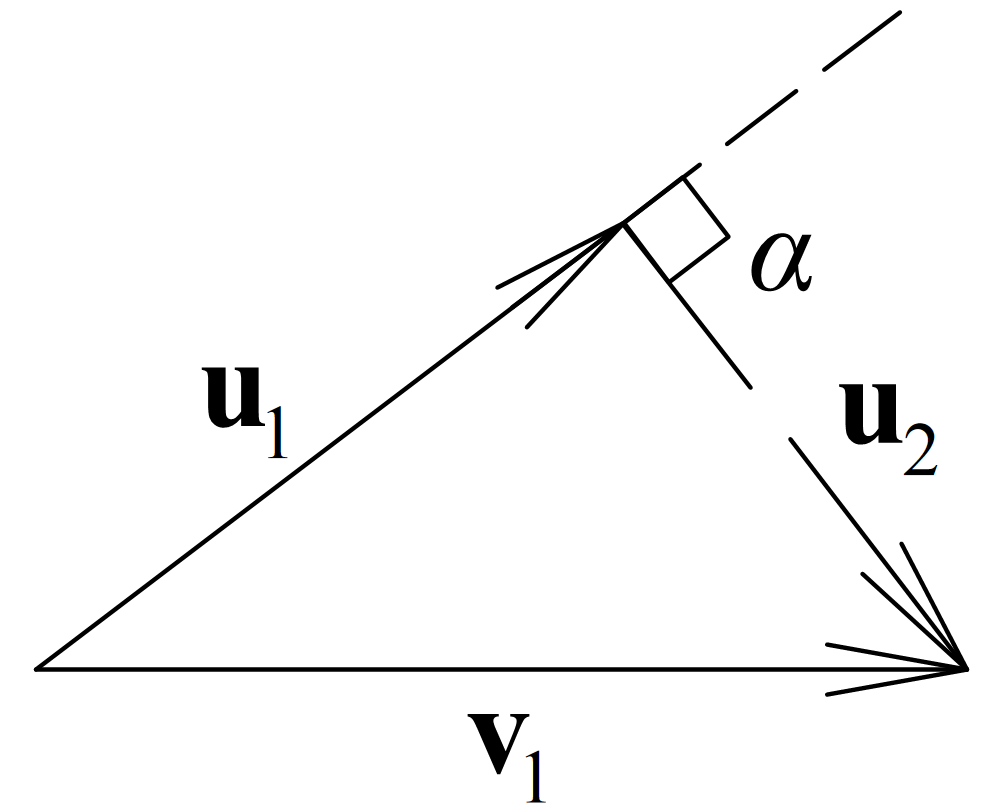
\includegraphics[scale = 0.22, keepaspectratio=true]{M4-VelocityDiagram}
\caption{Схема расчёта скоростей\label{fig:m4-velocity-triangle}} % ИЗМ: добавил "скоростей"
\end{figure}
% А вот здесь wrapfigure так и не заработал.


% Помоги, пожалуйста, придумать правильные названия для 4.1 и 4.2 --- там "схема расчета", сям "расчётная схема". Первый "для теории", второй "для лабы". Надо, чтобы было ясно, что они разные (и почему) | боюсь, что не могу помочь =( |

% ИЗМ: порядок слов, пояснено, что за теорема косинусов
Рассматривая совместно~\eqref{eq:m4-equal-balls-collision-v2zero} и~\eqref{eq:m4-equal-balls-collision-v2zero-energy}, по теореме косинусов для изображённого на рис.~\ref{fig:m4-velocity-triangle} треугольника скоростей получаем, что угол разлёта шаров есть %треугольник импульсов? не скоростей разве? | Верно, спасибо, я идиот.
\[
\alpha = \frac{\pi}{2}.
\]

\subsection{Описание экспериментальной установки}
Для измерения модулей скоростей шаров и определения направления их движения можно воспользоваться установкой, схема которой изображена на рис.~\ref{fig:m4-equipment}. В штативе закрепляется наклонный лоток таким образом, чтобы участок поверхности, с которой падает шар после скатывания по лотку, был расположен горизонтально. % ИЗМ: запятая после "шар" - явная опечатка, "с которой скатывактся" -> "с которой падает", чтобы не было повторений.

\begin{figure}[h]
\begin{center}
%\includegraphics[scale = 0.25, keepaspectratio=true]{M4-Equipment}
\end{center}
\caption{Cхема экспериментальной установки \label{fig:m4-equipment}}
\end{figure} % ИЗМ Это точно не "схема"

\subsection{Методика выполнения работы}

% ооох, как тут плохо - установка не описана, но они уже про лоток начинают.
% не стоит ли поменять разд. 4.3 и 4.4 местами? По-моему, \emph{очень даже} стоит. Посмотри, пожалуйста, со всей своей чудесной внимательностью, не порушит ли это чего-нибудь. | ты прав, так во всех лабах. поменяла | Отлично!

Дальность полета шара~$\vec l_1$ при падении на стол пропорциональна скорости~$\vec v_1$ на краю лотка:
\[
\vec l_1 = \vec v_1 t,
\]
% ИЗМ: тире, абзац после конца предложения
где $t$ "--- время падения шара, определяемое высотой лотка над столом.

% ИЗМ: сместить -> сместив
Направление вектора скорости~$\vec v_1$ совпадает с направлением вектора $\vec{AB}$, соединяющего точку~$A$ поверхности стола под краем лотка с точкой~$B$, в которую падает шар. Если на краю лотка поставить второй шар, сместив его на 3--5~\Units{мм} от траектории движения скатывающегося шара, то при скатывании по лотку первого шара в результате удара в движение приходят оба шара. (Подумайте, что будет при абсолютно упругом центральном ударе.) Отметив точки~$C$ и~$D$ падения шаров на стол, можно определить направление векторов скоростей~$\vec u_1$ и~$\vec u_2$ (рис.~\ref{fig:m4-impulse-diagram}). Длины отрезков~$AC$ и~$AD$ пропорциональны модулям скоростей шаров~$\vec u_1$ и~$\vec u_2$, так~как время падения шаров одинаково. %ИЗМ: "длина" -> "длины" | ИЗМ: "Подумайте, ... центральном ударе?" вопросительный знак заменила на точку

\begin{figure}[h]
\begin{center}
%\includegraphics[scale = 0.25, keepaspectratio=true]{M4-ImpulseDiagram}
\end{center}
\caption{Схема опыта \label{fig:m4-impulse-diagram}} % ИЗМ: "Схема опыта"? ://
\end{figure}

Таким образом, для проверки закона сохранения импульса при упругом столкновении двух шаров одинаковой массы необходимо проверить, равняется ли сумма векторов~$\vec{AC}$ и~$\vec{AD}$ (обозначим ее~$\vec{AB'}$) вектору~$\vec{AB}$, а угол разлета "--- $\pi/2.$





\subsection{Порядок выполнения работы}
\begin{enumerate}
  \item Приготовить в тетради две таблицы~\ref{tab:m4-first} и~\ref{tab:m4-second} для записи результатов измерений и вычислений.
      \begin{table}[h!]
      \caption{\label{tab:m4-first}}
      % ИЗМ: они потеряли обозначение градуса в последнем столбце
      \begin{center} %сделала шапку побольше, мне кажется, так красивее | Действительно
      \begin{tabular}{|c|c|c|c|c|} %мб стоит подлиннее таблицы сделать, скажи, как ты думаешь | Не вижу особых причин, вроде смотрится.
      \hline
      \multirow{2}*{\textnumero} & \multirow{2}*{$AB'$,~\Units{мм}} & \multirow{2}*{\hspace{3pt}$\MTDMean{AB'} \pm \Delta(AB')$,~\Units{мм}} & \multirow{2}*{$\alpha,~\Units{\degree}$} &  \multirow{2}*{\hspace{3pt}$\MTDMean{\alpha} \pm \Delta \alpha,~\Units{\degree}$} \\
      & & & & \\ \hline
      1 & & & & \\ \cline{1-2} \cline{4-4}
      2 & & & & \\ \cline{1-2} \cline{4-4}
      3 & & & & \\ \hline
      \end{tabular}
      \end{center}
      \end{table}

      \begin{table}[h!]
      \caption{\label{tab:m4-second}}
      % ИЗМ: почему-то нет 1, 2, 3 в левом ст-це, вроде нужны
      \begin{center}
      \begin{tabular}{|c|c|c|}
      \hline
      \multirow{2}*{\textnumero} & \multirow{2}*{$AB$,~\Units{мм}} & \multirow{2}*{\hspace{3pt}$\MTDMean{AB} \pm \Delta(AB)$,~\Units{мм}} \\
      & & \\ \hline %твои \right \left делают огромные отступы почему-то | Больше не буду. :)
      1 & & \\ \cline{1-2}
      2 & & \\ \cline{1-2}
      3 & & \\ \hline
      \end{tabular}
      \end{center}
      \end{table}

  \item Установите дугообразный лоток на высоте 5--10~\Units{см} и закрепите в штативе. Обратите внимание на горизонтальное положение нижнего края лотка.

  \item На столе под лотком в направлении полета шара положите лист миллиметровой бумаги и покройте его копировальной бумагой. Помните, что в ходе эксперимента миллиметровую бумагу со стола сдвигать нельзя.
  \item С помощью отвеса отметьте на миллиметровой бумаге точку~$A$ под краем лотка.
  \item Трижды запустите шар с верхнего края лотка. % ИЗМ: сдедал немного менее кривое предложение | мб "получившихся" -> "полученных"? | Да.
      Осторожно приподняв копировальную бумагу, обозначьте три полученных отметки от падения шаров как~$B^1, B^2, B^3.$
  \item Установите на краю лотка второй шар таким образом, чтобы вектор скорости первого шара не проходил через центр второго шара.
      % ИЗМ: запустите -> запустив
      Запустив первый шар с верхнего края лотка, получите отметки точек~$C$ и~$D$ падения обоих шаров на стол. Осторожно приподняв копировальную бумагу, обозначьте их как~$C^1$ и~$D^1$.

      \item
      % ИЗМ: добавил "точно", "как в п. 6" -> "согласно п. 6" | убрала "точно", зачем оно там? | <s> Война правок! </s> Окей.
      Опыт повторите~3~раза, каждый раз стараясь поставить шар на прежнее место. Полученные точки отмечайте согласно п.~6 с индексами соответственно~2 и~3.
      \item Возьмите лист миллиметровой бумаги с нанесенными на нем точками. С помощью циркуля и линейки постройте параллелограммы~$A C^1 {B}^{'1} D^1,$ $A C^2 {B}^{'2} D^2,$ $A C^3 {B}^{'3} D^3.$ % сделала {B}^{'1} вместо {B'}^{1}. все этро по-любому плохо смотрится, пусть хоть цифры на одном уровне будут | Хорошо.
      \item Измерьте линейкой отрезки~$A{B}^{'1},$ $A{B}^{'2},$ $A{B}^{'3}$ и занесите их значения в таблицу~\ref{tab:m4-first}. Рассчитайте по формулам раздела <<Введение>> среднее значение %поменяла обратно
расстояния~$AB'$ и по приведенной формуле абсолютную погрешность измерения
          \begin{equation} % Тут нужна запятая? | если я правильно поняла про что ты, то нет
          \label{m4:value-deltaABs}
          \Delta \MTDMean{AB'}\ = \frac{\left(AB'\right)_{\max} - \left(AB'\right)_{\min}}{2}.
          \end{equation}

    % Уместно ли "и" так выравнивать, Дин? | во-первых, у тебя сбилась нумерация, так как "и" - тоже формула, во-вторых, ИЗМ: раз уж ты везде убрал "и", то я здесь уберу, чтоб не мучиться, нигде больше эти "и" не писали между формулами, мб можно придумать что-то типа "рассчитайте \MTDMean{\alpha} и \Delta\MTDMean{\alpha} по приведенным ниже формулам:" | ИЗМ: имела смелость заменить все MIN и MAX на нижний регистр. кстати, не должны ли они быть курсивом, так как это название переменной? в Сивухине прямые |  Тогда прямые.
    % То, что сбилась нумерация, это лечится простановкой \nonumber около "и", я просто забыл. Но ок, к черту их все.
      \item Измерьте транспортиром углы~$\alpha_1,$ $\alpha_2,$~$\alpha_3$ и занесите их значения в таблицу~\ref{tab:m4-first}.
          % ИЗМ: убрана дурная последовательность "и".
           Рассчитайте
           \begin{align}
           \label{eq:m4-value-alpha}
           \MTDMean{\alpha}\ &= \frac{\alpha_{\max} + \alpha_{\min}}{2}, \\
           \label{eq:m4-value-dalpha}
           \Delta\MTDMean{\alpha}\ &= \frac{\alpha_{\max} - \alpha_{\min}}{2}.
           \end{align}

      \item Измерьте линейкой отрезки~$AB^1,$ $AB^2$,~$AB^3$ и занесите их значения в таблицу~\ref{tab:m4-second}.
           Рассчитайте
          \begin{align}
          \label{eq:m4-value-AB}
          \MTDMean{AB}\ &= \frac{\left(AB\right)_{\max} + \left(AB\right)_{\min}}{2}, \\
          \label{eq:m4-value-deltaAB}
          \Delta \MTDMean{AB}\ &= \frac{\left(AB\right)_{\max} - \left(AB\right)_{\min}}{2}.
          \end{align}
          \item % ИЗМ: сделал деепричастный оборот, значительно естественнее
           Сравнив отрезки~$AB$ и~$AB'$ и углы~$\alpha$ и~$\pi/2$, сделайте вывод о выполнении закона сохранения импульса в проведенном опыте. %", определите погрешость измерений." вроде уже везде определили, нет? | Вроде бы да.
          % ИЗМ: убрана дурная последовательность "и" | без "и" плохо из-за pi/2, придумай что-нибудь еще или верни обратно | Вернул, не заставляйте меня думать.
      \item Напишите заключение к работе.
\end{enumerate}

\subsection{Контрольные вопросы}
\begin{enumerate}
 \item При каких условиях импульс системы сохраняется?
 \item Почему необходима горизонтальная установка нижнего края лотка?
 \item
  Можно ли считать систему из шаров, сталкивающихся на горизонтальной части лотка, замкнутой?
  \item  % ИЗМ: В чем -> как | Изменила обратно, мне лично было бы проще ответить на их вопрос =) | Как хочешь, физик. :)
   В чем проявляется закон сохранения энергии в данной работе?
   \item Может ли человек, стоящий на идеально гладкой горизонтальной (ледяной) площадке, сдвинуться с места, не упираясь острыми предметами в лед?  % ИЗМ: добавил "главный", "действительно" | насчет "действительно": так как-то странно, мб лучше "Действительно ли можно таким образом поднять себя?" или как-то так | Угу. | ИЗМ: запятая "и себя, и своего коня"
   \item Главный герой книги Э.~Распе барон Мюнхгаузен рассказывает: <<Схватив себя за косичку, я изо всех сил дернул вверх и без большого труда вытащил из болота и себя, и своего коня, которого крепко сжал обеими ногами, как щипцами>>. Действительно ли можно таким образом поднять себя?
   \item В книге А.~Некрасова <<Приключения капитана Врунгеля>> описан следующий способ передвижения лодки: колесо приводят во вращение белки, несущиеся <<как бешеные одна за одной по ступенькам внутри колеса>> (беличьего колеса). Будет ли двигаться лодка с подобным двигателем? % Будет, вообще говоря, при достаточном весе и наглости белок, но у меня тут ощущение, что они хотят услышать "нет". :|
   \item Может ли висящая на паутине гусеница повернуться к наблюдателю другим боком?
   \item Небольшая лодка притягивается канатом к большому теплоходу. Почему теплоход не движется по направлению к лодке? % Движется он, движется, лгунишки...
   \item Чтобы сойти на берег, лодочник направился от кормы лодки к ее носовой части. Почему при этом лодка отошла от берега?
   \item Зачем рулевой во время движения лодки наклоняет тело в такт гребцам? % ИЗМ: Для чего -> Зачем
\end{enumerate}
\end{document} 